\documentclass[compress]{beamer}
\usepackage{etex}
\usepackage{subfig}
\usepackage{wrapfig}
\usepackage{bbold}
\usepackage{amsmath}
\usepackage{amssymb}

\usetheme{Orebro}

\newcommand{\lectureTitle}{Quadcopter Stabilization and Tracking}

%\addtolength{\bodyheight}{-2mm} 
%If you think \bodyheight is too tall, you can adjust it like this.

\definecolor{red}{rgb}{1,0,0}\newcommand{\red}{\color{red}}
\definecolor{darkred}{rgb}{0.60,0.11,0.11}\newcommand{\darkred}{\color{darkred}}
\definecolor{darkgreen}{rgb}{0.4,1.0,0.4}\newcommand{\darkgreen}{\color{darkgreen}}
\definecolor{darkyellow}{rgb}{1.0,0.8,0.0}\newcommand{\darkyellow}{\color{darkyellow}}
\definecolor{darkblueone}{rgb}{0.2,0.2,1.0}\newcommand{\darkblueone}{\color{darkblueone}}
\definecolor{gray}{rgb}{0.8,0.8,0.8}\newcommand{\gray}{\color{gray}}
\definecolor{darkgray}{rgb}{0.6,0.6,0.6}\newcommand{\darkgray}{\color{darkgray}}
\definecolor{darkbluea}{rgb}{0.13,0.13,0.44}\newcommand{\darkbluea}{\color{OruBlue}}
\definecolor{darkblue}{rgb}{0.18,0.23,0.53}\newcommand{\darkblue}{\color{darkblue}}
\definecolor{white}{rgb}{1.0,1.0,1.0}\newcommand{\white}{\color{white}}
\definecolor{black}{rgb}{0.0,0.0,0.0}\newcommand{\black}{\color{black}}
\definecolor{ugreen}{rgb}{0.24,0.62,0.24}\newcommand{\ugreen}{\color{ugreen}}
\definecolor{lgreen}{rgb}{0.88,0.91,0.88}\newcommand{\lgreen}{\color{lgreen}}
\definecolor{ured}{rgb}{0.7,0.2,0.2}\newcommand{\ured}{\color{ured}}
\definecolor{lred}{rgb}{0.85,0.6,0.6}\newcommand{\lred}{\color{lred}}
\definecolor{reallylightblue}{HTML}{D4EAFF}\newcommand{\reallylightblue}{\color{reallylightblue}}
\definecolor{lightgray}{HTML}{A7A7A7}\newcommand{\lightgray}{\color{lightgray}}
\definecolor{orange}{HTML}{FF9700}\newcommand{\orange}{\color{orange}}
\definecolor{mygray}{RGB}{185,220,255}\newcommand{\mygray}{\color{mygray}}

\newcommand{\at}{\makeatletter @\makeatother}

\newcommand{\mymovie}[3]{
\begin{center}
\movie[
           width=#1\textwidth,
           autostart
%           poster,
%           loop
           ]
           {
             \centering
             \hspace{-0.1cm}\includegraphics[width=#1\textwidth]{#2}
           }
          {#3}
\end{center}
}


\newcommand{\mymovienocenter}[3]{
\movie[
           width=#1\textwidth,
           autostart
%           poster,
%           loop
           ]
           {
             \centering
             \hspace{-0.1cm}\includegraphics[width=#1\textwidth]{#2}
           }
          {#3}
}

\newcommand{\OruBlue}{\color{OruBlue}}

\newcommand{\changespace}[1]{\renewcommand{\baselinestretch}{#1}\normalsize}

\usepackage{savesym}
\usepackage{xcolor,colortbl}
\usepackage{multimedia}
%\usepackage{CJKutf8}
\usepackage[english]{babel}
%\usepackage{eurosans}
%\usepackage{eurosym}
\usepackage{alltt}
\usepackage{calc}
\usepackage{marvosym}
\usepackage[ruled,vlined]{algorithm2e}
\usepackage{pstricks}
\usepackage[thicklines]{cancel}
\usepackage{empheq}
\usepackage[absolute,overlay]{textpos}

\savesymbol{Cross}
\usepackage{bbding}
\restoresymbol{TXF}{Cross}

\usepackage{tikz}
% \usepackage[absolute,overlay]{textpos}
% \textblockorigin{0mm}{0mm}

\newcommand{\transboxnocenter}[2]{
  \begin{center}
    \fbox{
      \begin{minipage}{#1\textwidth}\vspace{0.1cm}
        #2 \vspace{0.1cm}
      \end{minipage}
    }
  \end{center}
}

\newcommand{\transbox}[2]{
  \begin{center}
    \fbox{
      \begin{minipage}{#1\textwidth}\vspace{0.1cm}
        \centering #2 \vspace{0.1cm}
      \end{minipage}
    }
  \end{center}
}

\newcommand{\nontransbox}[2]{
  \begin{center}
    \fcolorbox{black}{white}{
      \begin{minipage}{#1\textwidth}\vspace{0.1cm}
        \centering #2 \vspace{0.1cm}
      \end{minipage}
    }
  \end{center}
}


\DeclareMathOperator*{\argmin}{arg\,min}
\DeclareMathOperator*{\argmax}{arg\,max}
\newcommand{\mbm}[1]{{\bf #1}}
\newcommand{\dba}[1]{{\OruBlue{\bf #1}}}
\newcommand{\dbb}[1]{{\OruBlue{\bf{\em #1}}}}
\newcommand{\mybox}[2]{
%
	\begin{center}
	%\vspace{-0.2cm}
	\begin{tabular}{|c|}
	\hline
	\begin{minipage}{#1\textwidth}\vspace{0.3cm}
	\centering
	\emph{
	#2
	}
	\vspace{0.3cm}\end{minipage}\\
	\hline
	\end{tabular}
	%\vspace{-0.2cm}
	\end{center}
%
}

\newcommand{\graybox}[1]{
\fboxrule=0pt
\begin{center}
\vspace{0.3cm}
\noindent
\fcolorbox{black}{mygray}{\parbox{0.94\columnwidth}{\vspace{0.3cm}
\begin{minipage}{0.92\columnwidth}\centering
#1
\end{minipage}
\vspace{0.3cm}
}}
\end{center}
\vspace{0.3cm}
}

% gray box
\newcommand{\gbox}[1]{
  \begin{center}
    \fcolorbox{black}{gray}{
      \begin{minipage}[b]{0.98\textwidth}
        \begin{center}
          %\vspace{2mm}
          \begin{minipage}{0.97\textwidth}
            #1 
          \end{minipage}
          \vspace{2mm}
        \end{center}
      \end{minipage}
    }
  \end{center}
}

\newcommand{\wbox}[1]{
  \begin{center}
    \fcolorbox{black}{white}{
      \begin{minipage}[b]{0.98\textwidth}
        \begin{center}
          %\vspace{2mm}
          \begin{minipage}{0.97\textwidth}
            #1 
          \end{minipage}
          \vspace{2mm}
        \end{center}
      \end{minipage}
    }
  \end{center}
}

\mode<presentation>
{
%\useoutertheme{infolines}
\setbeamertemplate{footline}
{
  \hbox{%
  \begin{beamercolorbox}[wd=.9\paperwidth,ht=2.25ex,dp=1ex,center]{title in foot}%
  \usebeamerfont{title in foot}{\OruBlue\copyright{} 2016 \insertshortauthor{} / \"Orebro University -- \url{aass.oru.se}} \end{beamercolorbox}%
\begin{beamercolorbox}[wd=.1\paperwidth,ht=2.25ex,dp=1ex,right]{date in head/foot}%
    \usebeamerfont{date in head/foot}{\OruBlue\insertframenumber{} / \inserttotalframenumber\hspace*{2ex}}
  \end{beamercolorbox}}%
  \vskip0pt%
}
}

% ===========================================================================
\title{Robot Control Project}
\subtitle{\lectureTitle{}}
\author[Chittaranjan Srinivas Swaminathan and Anders Wikstr\"{o}m]{Chittaranjan S Srinivas and Anders Wikstr\"{o}m\\\url{chitt@live.in}\\\url{anders.wikstrom.88@gmail.com}\\\vspace{0.2cm}School of Science and Technology\\\vspace{0.1cm}\"Orebro University, Sweden}

\date{\centering
\vspace{1cm}

\includegraphics[height=45pt]{themeFig/Logo_txt_runt_farg-big.png}
}


%Optional extra graphics on the title page
\titlegraphic{%
  \colorbox{reallylightblue}{\parbox[t][\paperheight][c]{\linewidth}
    {
        %\vspace{1.3cm}
        \begin{center}
        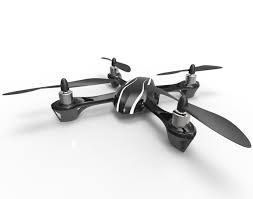
\includegraphics[width=\linewidth]{quadrotor.jpg}
        \end{center}
      %WITH FUNDER LOGO(S)
      %WITH CONTRIBUTORS
      % \vspace{0.3cm}
      % {\OruBlue $^\star$}
      % \begin{minipage}{0.9\linewidth}\changespace{0.6}
      % \scalebox{.6}{{\OruBlue{\em Lecture in partial achievement}}}
      % \scalebox{.6}{{\OruBlue{\em of Associate Professorship}}}
      % %$\;$ 
\includegraphics[width=0.6\linewidth]{themeFig/kk_eng_colour_tif.png}
      % \end{minipage}
    }%
  }%
}

% %Optional extra graphics on the title page
% \titlegraphic{%
% %  \colorbox{OruBlue}{\parbox[t][\paperheight][c]{\linewidth}
%   \colorbox{reallylightblue}{\parbox[t][\paperheight][c]{\linewidth}
%     {
%       {\flushright
%         \includegraphics[width=\linewidth]{newfig/tl-fragment.png}\\
%       }
%       \vspace{0.3cm}
%       {\black \scalebox{.6}{$^\star$ {\em Contributors:}}}\\\vspace{-0.15cm}
%       {\black $\;\;$ \scalebox{.6}{H.~Andreasson, M.~Cirillo, T.~Stoyanov}}%\\\vspace{-0.15cm}
%     }%
%   }%
% }


% ===========================================================================
\begin{document}
\maketitle

\section{Outline and Introduction}

\frame{
  \frametitle{Introduction}
  
\dba{Goal}: Build a stability and tracking controller for a quadcopter.
\begin{itemize}
\item Stability: maintain orientation and hover at a particular altitude.
\item Tracking: follow trajectories given.
\end{itemize}
\dba{Subgoal}: Build a simulator for the quadrotor in matlab.\\
\dba{Result}: Built an inverse dynamics controller that can
stabilize the quadcopter and track paths.
}

\frame{
\frametitle{Outline}
\vspace{0.5cm}
{

\begin{itemize}
\item Introduction
\item Key concepts
\item Controller design
\item Results
\end{itemize}
%% this can be used to select a different font.
%%\fontsize{6}{2}\selectfont

}
}

\section{Key concepts}
\frame{
  \frametitle{Forces from propellers}
  \begin{tabular}{l r}
   $ \dba{T_{B}} = k \begin{bmatrix}0 \\ 0\\ \sum
      \limits_{i=1}^{4} \omega_i^2 \end{bmatrix} $
& \onslide<1-> 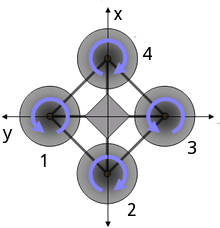
\includegraphics[scale=0.5]{../Report/quadrotor.png}\\
  \end{tabular}
}

\frame{
  \frametitle{Torques from propellers}
  \begin{tabular}{l r}
$ \tau_\theta = L (k\omega_2^2 - k\omega_4^2) $

& \onslide<1-> 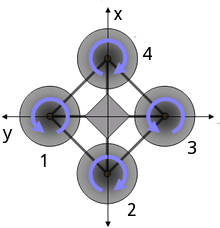
\includegraphics[scale=0.5]{../Report/quadrotor.png}\\
  \end{tabular}
}

\frame{
  \frametitle{Torques from propellers}
  \begin{tabular}{l r}
$ \tau_\phi = L (k\omega_1^2 - k\omega_3^2) $

& \onslide<1-> 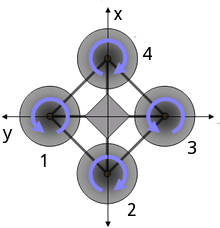
\includegraphics[scale=0.5]{../Report/quadrotor.png}\\
  \end{tabular}
}

\frame{
  \frametitle{Torques from propellers}
  \begin{tabular}{l r}
$ \tau_\psi = b\ (\omega_1^2 - \omega_2^2 + \omega_3^2 -
\omega_4^2) $

& \onslide<1-> 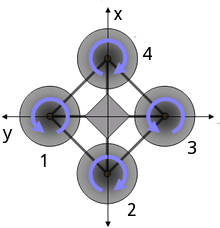
\includegraphics[scale=0.5]{../Report/quadrotor.png}\\
  \end{tabular}
}

\frame{
  \frametitle{Equations of motion}
  \begin{itemize}
    \item Linear: $ m \mathbf{\frac{d^2x}{dt^2}} = \mathbf{G} + \mathbf{^BR_IT_{B}} +
      \mathbf{F_{D}} $
    \item Rotational: $\mathbf{\tau_B} = \mathbf{J\frac{d\omega}{dt}} + \mathbf{\omega} \times (\mathbf{J\omega})$

  \end{itemize}
}

\section{Controller Design}

\frame{
  \frametitle{Inverse Dynamics formulation}
 In matrix form ...
    $$ \mathbf{F} = \mathbf{M}\mathbf{x''} + \mathbf{S} -\mathbf{G} - \mathbf{F_D} $$
\begin{itemize}    
\item $ \mathbf{M} = \begin{bmatrix} m\mathbf{I} && \mathbb{O}\\ \mathbb{0}&&
  \mathbf{J}\end{bmatrix} $ and $ \mathbf{S} = \begin{bmatrix} \mathbb{0}_{3\times1} \\ \mathbf{\omega} \times (\mathbf{J\omega}) \end{bmatrix} $ \\

\item $ \mathbf{G} = \begin{bmatrix} 0 \\ 0\\ -mg\\ 0\\ 0\\
    0 \end{bmatrix} $ and $ \mathbf{F_D} = \begin{bmatrix} -k_d \mathbf{x'}\\
  \mathbb{0}_{3\times1} \end{bmatrix} $
\end{itemize}
}

\frame{
  \frametitle{Inverse Dynamics Formulation}
Forces in the world/inertial frame...
$$ \mathbf{F} = \mathbf{M}(\mathbf{a_r} + \mathbf{K_p}\mathbf{e_p} +
\mathbf{K_d}\mathbf{e_v}) + \mathbf{S} -\mathbf{G} - \mathbf{F_D} $$

Where, 
$$ \mathbf{u} = e'' = a_r - a_c =
-\mathbf{K_p}\mathbf{e_p} - \mathbf{K_d}\mathbf{e_v} $$
and

$$ \begin{bmatrix} \mathbf{y'} \\ \mathbf{y''} \end{bmatrix}
= \begin{bmatrix} \mathbb{0} && \mathbf{I} \\ \mathbb{0} &&
  \mathbb{0} \end{bmatrix} \begin{bmatrix} \mathbf{y} \\
  \mathbf{y'}\end{bmatrix} + \begin{bmatrix} \mathbb{0}  \\
  \mathbf{I} \end{bmatrix} \mathbf{u}$$

}

\frame{
  \frametitle{Small angle approximation - force equation}
  We could reduce the Rotation matrix to ...
  $$  \mbm{^BR_I} = \begin{bmatrix} 1 && -\psi && \theta \\ \psi && 1 && -\phi \\
  -\theta && \phi && 1 \end{bmatrix} $$

And hence, 

$$ f_x  = \theta\ f_{th} $$
$$ f_y = -\phi\ f_{th} $$
}

\section{Results}

\frame{
  \frametitle{Helical trajectory - error graphs}
  \begin{figure}[H]
    \begin{tabular}{cc}
      \subfloat[Error]{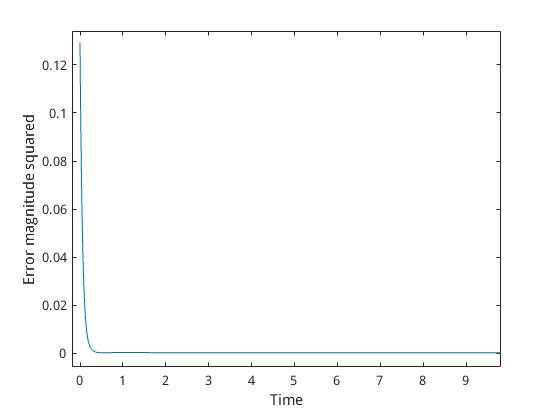
\includegraphics[width=1.5in]{../Report/error4.jpg}} &
                                                                  \subfloat[Orientation error]{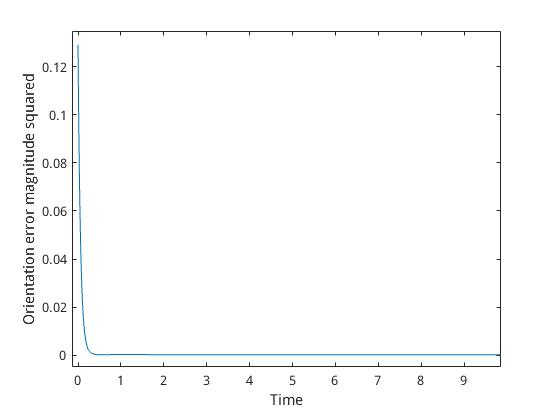
\includegraphics[width=1.5in]{../Report/oerror4.jpg}} \\
      \subfloat[Position error]{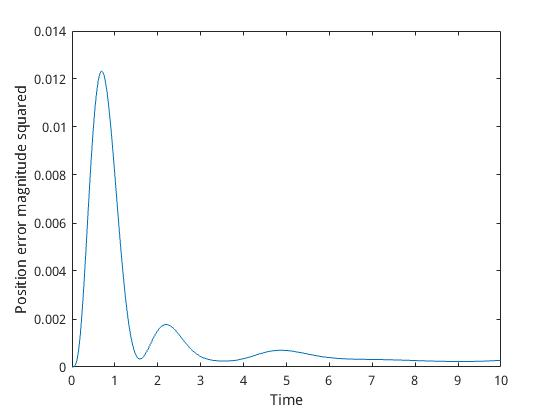
\includegraphics[width=1.5in]{../Report/perror4.jpg}} &
                                                                            \subfloat[Velocity error]{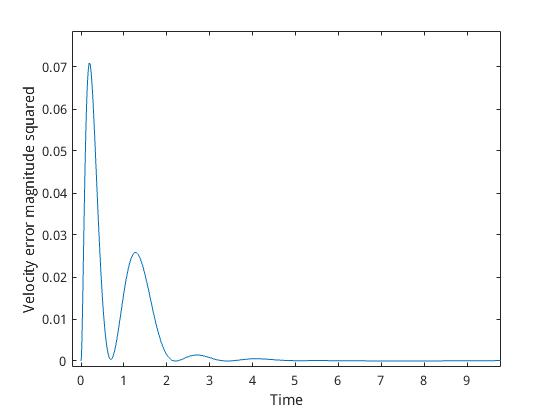
\includegraphics[width=1.5in]{../Report/verror4.jpg}} \\
    \end{tabular}
  \end{figure} 
}

\frame{
  \frametitle{Another goal - error graphs}
  \begin{figure}[H]
    \begin{tabular}{cc}
      \subfloat[Error]{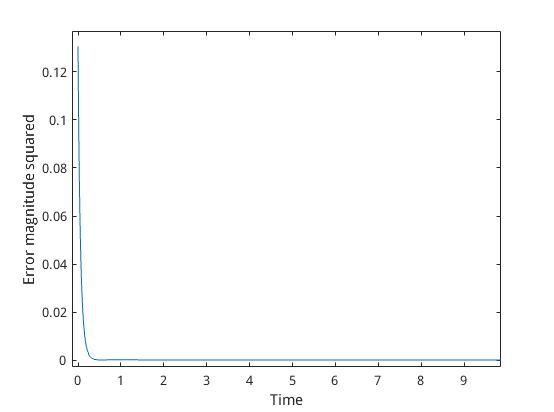
\includegraphics[width=1.5in]{../Report/error3.jpg}} &
                                                                  \subfloat[Orientation error]{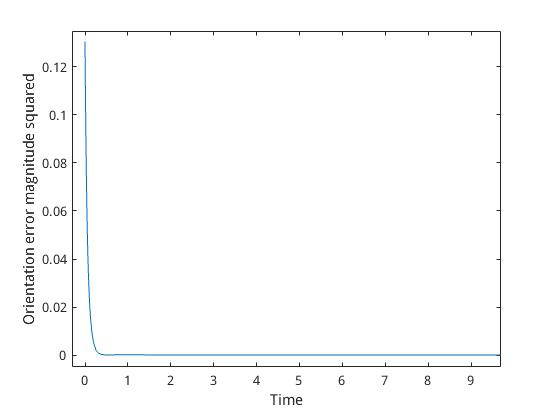
\includegraphics[width=1.5in]{../Report/oerror3.jpg}} \\
      \subfloat[Position error]{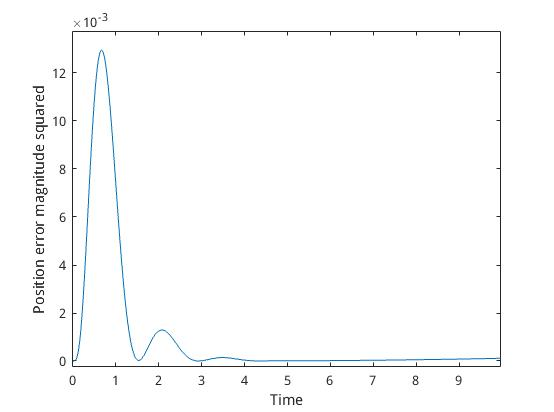
\includegraphics[width=1.5in]{../Report/perror3.jpg}} &
                                                                            \subfloat[Velocity error]{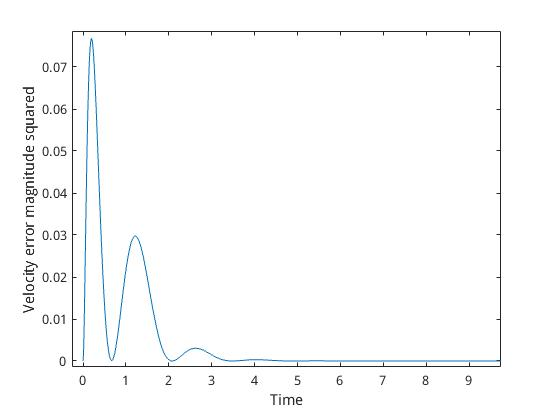
\includegraphics[width=1.5in]{../Report/verror3.jpg}} \\
    \end{tabular}
  \end{figure} 
}

\end{document}


